\documentclass[12pt]{article}

% Set up data, if you need to add a package, go here
%Adapted from Adapted from UWA Engineering Final Year Project.


%\usepackage[utf8]{inputenc}
\usepackage[x11names,dvipsnames,svgnames,table]{xcolor}

% general incantations
\usepackage[export]{adjustbox}
\usepackage{afterpage}

\usepackage{graphicx}
\usepackage{placeins}
\usepackage{pdfpages}
\usepackage{algorithm2e}
\usepackage{array}
\usepackage{booktabs}
\usepackage[most]{tcolorbox}
\usepackage{calligra}
\usepackage{caption}
\usepackage{datetime}
%\usepackage{dblfnote}
\usepackage{dirtytalk}
\usepackage{dsfont}
\usepackage{etex}
\usepackage{fancyhdr}
\usepackage{fix-cm}
\usepackage[T1]{fontenc}
\usepackage{textcomp,gensymb} %for \degree C symbol
\usepackage{graphicx}
\usepackage{lipsum}
\usepackage{listings}
\usepackage{transparent}
\usepackage[everyline=true,framemethod=tikz]{mdframed}
\usepackage{mparhack}
\usepackage{multicol}
\usepackage{multirow}
\usepackage{parskip}
\usepackage{lscape}
\usepackage{pdflscape}
\usepackage{pdfpages}
\usepackage{placeins}
\usepackage[document]{ragged2e}
\usepackage{rotating}
\usepackage{setspace}
\usepackage{subcaption}
\usepackage{threeparttable}
\usepackage[normalem]{ulem}
\usepackage{verbatim}
\usepackage{soul} %highlighting, strike through etc.

%Automated appendices
\usepackage[titletoc,title,header]{appendix} %advanced functionality

%language settings
\usepackage[utf8]{inputenc}
\usepackage[australian]{babel}
\usepackage{csquotes}

%page setup
%this where we adjust the binding offset, if relevant
\usepackage[a4paper]{geometry}
\usepackage{lastpage} % for page 1 of n footers

%cross referencing
\usepackage{hyperref}

%maths stuff
\usepackage{amsmath}
\usepackage{mathtools}

\setcounter{secnumdepth}{5}

%lists
\usepackage{enumitem}

%working collaboratively
\usepackage[backgroundcolor=yellow]{todonotes}

% bibliography file using harvard
\usepackage[round, sort, numbers, authoryear]{natbib}

%glossary for acronyms
\usepackage[acronym,nonumberlist,toc,section=subsection,numberedsection=nolabel]{glossaries} 
\makeglossaries

%line spacing
\linespread{1.25}

\usepackage{natbib}

\begin{document}

\thispagestyle{empty}
\setlength\headheight{0pt} 
\begin{center}

\begin{center}

\includegraphics[width=0.65\linewidth]{images/UL_logo.jpg}            
\end{center}	

        \vspace{0.25cm}
        {\scshape\LARGE University of Limerick \par}
        \vspace{0.25cm}
        {\scshape\Large CS4157 Software Quality\par}
        \vspace{0.5cm}

        {\Large\bfseries The Role \& Importance of Testing in Facilitating the Development of Quality Software\par}
        
        \vspace{0.5cm}
        {\Large\itshape Niall Dillane\par}
        CSIS
        \vspace{0.25cm}

\vspace{1cm}
Submitted to\par
Dr. Valentine Casey \\
CSIS\par
\vspace{1.5cm}
\large
\today

\end{center}

\clearpage
\restoregeometry
\justify

\section*{Abstract}

Testing is an often neglected stage of the software development process, garnering less praise and compensation for its workers. Throughout this paper, we will research and demonstrate the various aspects of testing, as well as its importance in developing high quality systems. 

\pagebreak


\tableofcontents
\pagebreak



\section{Introduction}

Software Testing is the investigation of software for the purpose of finding defects and providing feedback on the quality of the product (\Citealt{kaner2006exploratory}). This typically involves running the program --- either manually or automatically with some kind of script --- and providing input with the intent of finding defects (colloquially known as bugs), or rather proving that there are no bugs. Of course, it is impossible to prove that a piece of software is entirely bug free (\Citealt{pan1999software}), at least if it has any degree of complexity, but testing aims to provide a reasonably complete picture of the state of the software and an avenue to reducing defects.

Testing has become more prominent in recent years (\Citealt{tuteja2012research}), but I believe it still does not get the credit it deserves. Testing is a very broad area, which is key at each stage of the software development process: from specification, to implementation, to maintenance. As it consumes 40-50\% of development efforts (\Citealt{tuteja2012research}), it warrants significant consideration and planning from the beginning, so as to minimise costs and time needed later on.



\section{Dynamic Analysis in Verification and Validation}
Research and discuss the role and importance of dynamic analysis in the verification and validation of software and the essential part it plays in facilitating quality.

There are two different types of analysis in software testing: those are static and dynamic analysis. 

Static analysis simply involves analysing a piece of software without actually running it (\Citealt{wichmann1995industrial}). This can entail human review of code in a text editor, tools used to provide statistics e.g. lines of code per file, or the use of a compiler. This can be useful in certain circumstances, such as finding security vulnerabilities in a codebase (\Citealt{livshits2006improving}) and is naturally quicker than walking through a program, but generally it is limited from a "user experience" point of view.

Dynamic analysis is based on system execution, often using tools to automate the process (\Citealt{ghahrai2018static}). There are various stages, from individual unit tests of small portions of the system, to integrating these units and the system overall. Dynamic testing provides a more complete picture of the state of the system, and is a more "real life use" approach. This can be time consuming, and so more and more automation is sought out, but one must be wary of the false sense of security these tools can provide.

Verification and Validation are related concepts in software testing. In whole, they describe the process of: identifying if the system has satisfied the specification provided (verification); and determining if that specification is what the customer really wants or needs (validation). In short, verification answers the question: "Are we building the system right?", and validation answers "Are we building the right system?" (\Citealt{boehm1984verifying}). 

Dynamic verification involves, as outlined previously, executing the code. At this point, developers wish to identify if the system has been built to specification, conducting a review of the program in various ways. These can be testing in the small --- checking if inidividual functions perform as expected --- up to testing the system as a whole, by executing modules and checking that they interact as expected. Non-functional requirements (discussed more in Section~\ref{reqs}) may also be tested, such as stress-testing a server to see how many users it can handle.

Dynamic validation is an even higher level of testing (acceptance testing), wherein the development team and external stakeholders walk through the product and use it as a user would. This is black box testing (see Section~\ref{blackwhitebox}), as the testers are performing these actions without looking at the internal workings of the system. A purely surface view.

It's important because.



\section{Functional and Non-Functional Requirements} \label{reqs}
Clearly outline and define what Functional and Non-Functional Software Requirements are and in your discussion compare and contrast the differences between them

\subsection{How to Test}
Research and discuss how Functional Software Requirements and Non- Functional requirements can be successfully tested and define the differences in approach required by each



\section{Software Testing Process}
Outline and discuss the key stages in the software testing process

\subsection{Unit Testing}

\subsection{Integration Testing}

\subsection{Regression Testing}

\subsection{System Testing}

\subsection{Acceptance Testing}



\section{Effective Test Strategy}
Research and define the principles of an effective test strategy.

\subsection{Documented Test Procedures}
Consider and discuss the role and importance of having documented test procedures in place to facilitate effective testing

\subsection{Test Plan}
Research and outline the purpose, importance and content of a test plan



\section{White Box and Black Box Testing} \label{blackwhitebox}
Define and discuss the importance of utilizing both white box and black box testing



\pagebreak
\section{Sample Table}
\begin{table}[ht!]
\centering
    
	\caption{Comparison \textit{p} values}
	\begin{tabular}{ |l|c|c|}	
		\hline		
		\textbf{Attribute} & \textbf{\textit{p-value}} & \textbf{Significant} \\ \hline
		Model A	 & 0.0521 & N \\ \hline
		Model B  & 0.6171 & N \\ \hline 
		Model C  & <0.00001 & Y \\ \hline 
	\end{tabular}
	\label{tab:pvalues}
\end{table} 


\subsubsection{Sample Figure}
\begin{figure}[ht!]
 	\centering
 	\caption{Perceptron (Artificial Neural Network)}
 	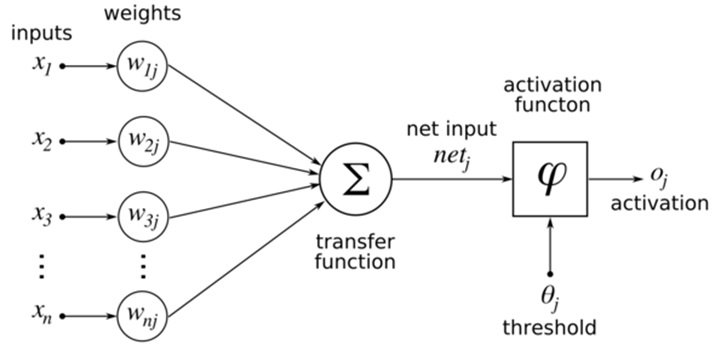
\includegraphics[width=0.7\linewidth]{images/ANN.jpg}
 	\label{lab:perceptron}
 \end{figure}
\pagebreak




%prints bibliography from bibliography file.
\bibliographystyle{agsm}
\renewcommand{\bibname}{References} % changes the header; default: Bibliography
\bibliography{bibliography.bib} % with extension

\end{document}
